%%
%% Apresentação da Ideia do Projeto.tex
%% Projeto Oficinas de Integração 3
%% Created by Leonardo Winter Pereira and Lucas Zimmermann Cordeiro on 10.03.2016
%% Copyright (C). All rights reserved
%%

\documentclass[hyperref={pdfpagelabels=false}]{beamer}

\usepackage[brazil, portuges]{babel} % pacote português brasileiro
\usepackage[utf8]{inputenc} % pacote para acentuação direta
\usepackage{lmodern}
\usetheme{CambridgeUS}

\title{Oficinas de Integração III}
\author{Leonardo Winter Pereira \newline Lucas Zimmermann Cordeiro \newline Luís Felipe Mazzuchetti Ortiz}
\date{\today}

\begin{document}

    \begin{frame}
    \titlepage
    \end{frame}

    \begin{frame}\frametitle{Índice}
        \tableofcontents
    \end{frame}

    \section{Dalle Pad}

        \begin{frame}\frametitle{Dalle Pad}

            \begin{figure}
                    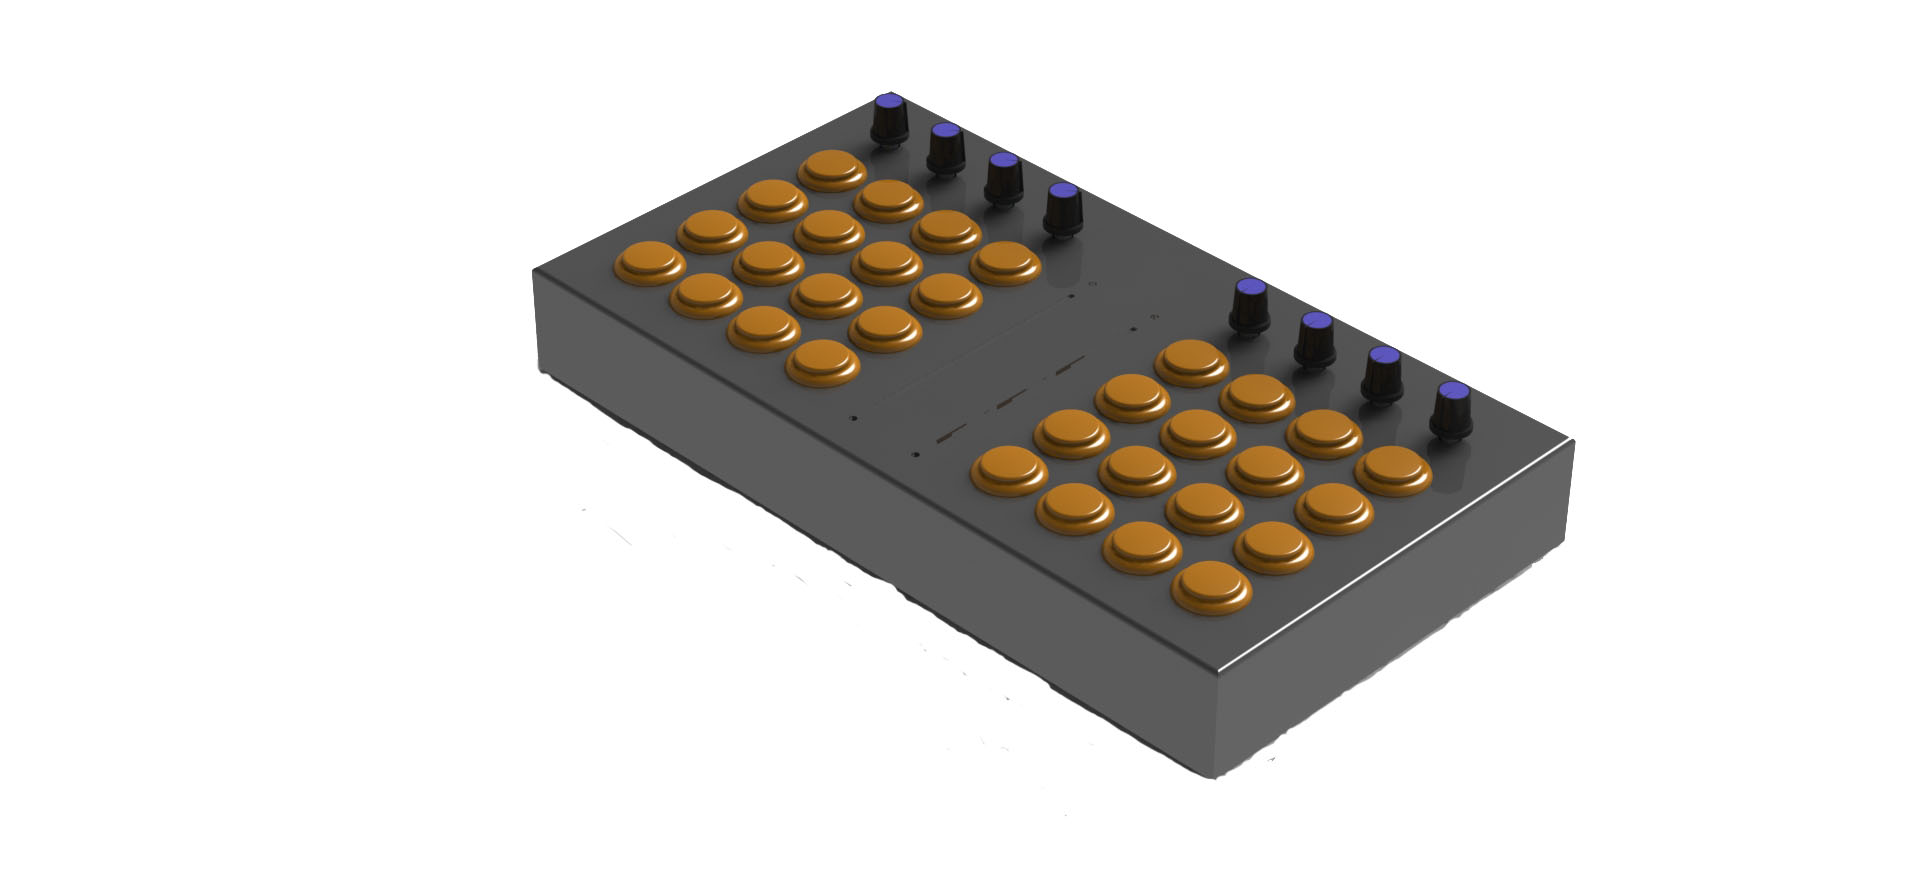
\includegraphics[scale=0.15]{Imagens/DallePad360.jpg}
                    \caption{Dalle Pad - O Gadget que te transforma em um DJ}
            \end{figure}

        \end{frame}

        \subsection{Equipe}

            \begin{frame}\frametitle{Equipe}

                \begin{figure}
                    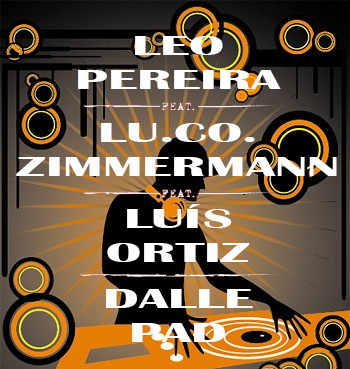
\includegraphics[scale=0.5]{Imagens/Equipe.png}
                \end{figure}

            \end{frame}
            
        \subsection{O que é}
        
             \begin{frame}\frametitle{O que é}

                Without title something is missing.

            \end{frame}

\end{document} 